\documentclass[12pt,a4paper]{article}
\usepackage[fontset=none]{ctex}
\setCJKmainfont[AutoFakeBold=2,AutoFakeSlant=.2]{SimSun}
\setCJKmonofont{SimSun}
\usepackage[margin=1in]{geometry}
\usepackage{amsmath,amssymb,bm}
\usepackage{booktabs,array}
\usepackage{graphicx}
\usepackage{hyperref}
\usepackage{fancyhdr}
\hypersetup{colorlinks,linkcolor=blue,citecolor=blue,urlcolor=blue}
\setlength{\headheight}{15pt}
\setlength{\emergencystretch}{3em}
\pagestyle{fancy}
\fancyhf{}
\fancyhead[L]{二维浅水方程：DTA 与强约束 4D-Var}
\fancyhead[R]{\thepage}
\newcommand{\Q}{\mathbf{Q}}
\newcommand{\q}{\mathbf{q}}
\newcommand{\LL}{\bm{\Lambda}}
\newcommand{\R}{\mathbb{R}}
\newcommand{\trans}{^{\mathsf T}}
\title{方法二：二维浅水方程的离散后伴随（DTA）\\
\large 精确离散梯度、检查点重算与强约束 4D-Var 数值验证}
\author{杨鹏亮}
\date{2026年10月16日}

\begin{document}
\maketitle
\begin{abstract}
本文完整描述现行代码的 discretize-then-adjoint（DTA，先离散、后求伴随）方法。
前向模式采用守恒变量、Rusanov 有限体积通量和 SSP-RK2 时间推进；离散伴随逐一
转置数值通量、边界索引映射及 RK2 组合，得到离散观测代价关于初始全状态的梯度。
现行 C 实现由 Tapenade 自动生成观测代价的反向代码，采用其原生二项式检查点调度，
以独立于观测步距的快照预算控制重算与存储，避免保存全窗口的所有 RK 阶段。
4D-Var 在白化控制空间使用对称余弦谱背景协方差平方根及 SciPy L-BFGS-B 求解。
固定步长下，所有阶段均检查正水深、有限性和二维 CFL 条件，无效试探不做裁剪。
在原始实验不变的对照中，新优化器以 16 次迭代收敛；在新的 $60\times60$ 相关背景误差
孪生实验中，同化窗水深 RMSE 降低 $87.5\%$，窗外自由预报降低 $97.4\%$，未参与同化的
测点残差 RMS 降低 $82.9\%$。文中同时报告梯度、守恒和内存检查，并明确这些结果的
适用范围。本文件只讨论 DTA，不改写或替代 ATD 推导。
\end{abstract}
\tableofcontents
\clearpage

\section{问题定义与离散优化目标}
\label{sec:dta-problem}

\subsection{状态、网格和强约束}

在矩形区域 $[0,L_x]\times[0,L_y]$ 上采用均匀网格，
$\Delta x=L_x/N_x$、$\Delta y=L_y/N_y$，单元中心坐标为
$x_i=(i+\tfrac12)\Delta x$、$y_j=(j+\tfrac12)\Delta y$。
记 $N=N_xN_y$，每个单元的守恒状态及速度为
\begin{equation}
 \q_{i,j}=(h,m_x,m_y)\trans,\qquad m_x=hu,\quad m_y=hv,
 \qquad u=m_x/h,\quad v=m_y/h.
 \label{eq:dta-state}
\end{equation}
全场 $\Q\in\R^{3N}$ 按 $h,hu,hv$ 三个分量连续存储，每个分量内的索引为
$k=i+N_xj$。这里 $h$ 是水深，不是自由表面相对静水面的扰动。
代码中重力加速度 $g=9.81$，无地形、科氏力、摩擦或外源项。

一次数值时间步记为 $\mathcal M$，固定步长 $\Delta t$，则
\begin{equation}
 \Q^{n+1}=\mathcal M(\Q^n),\qquad n=0,\ldots,N_t-1.
 \label{eq:dta-model-map}
\end{equation}
强约束 4D-Var 只调整 $\Q^0$，窗口内没有独立的模型误差控制量。
设每隔 $s$ 步观测一次，共 $C$ 个观测时刻，$n_c=cs$，$N_t=Cs$。
所有时刻的观测共同约束同一个初值，\emph{不是}依次运行 $C$ 个独立同化窗口。

\subsection{观测与背景项}

$H:\R^{3N}\to\R^{M}$ 在固定的 $M$ 个单元提取水深，
$(H\Q)_p=h_{o_p}$。观测误差独立，$R=\sigma_o^2 I_M$。
在背景误差协方差 $B$ 正定时，常规目标函数为
\begin{equation}
 J_x(\Q^0)=\frac12(\Q^0-\Q_b)\trans B^{-1}(\Q^0-\Q_b)
       +J_o(\Q^0),
 \qquad
 J_o=\frac12\sum_{c=1}^{C}\|H\Q^{n_c}-\mathbf y_c\|_{R^{-1}}^2.
 \label{eq:dta-physical-cost}
\end{equation}
这是标准的强约束变分同化形式\cite{asch2016data}。本实现采用欧氏离散向量内积；
上述代价没有额外乘 $\Delta x\Delta y$ 或 $\Delta t$，伴随转置也按同一约定定义。
因此不能在梯度中另加一个面积或时间权重。

实际求解的是白化控制 $\mathbf z\in\R^{3N}$：
\begin{equation}
 \Q^0=\Q_b+L\mathbf z,\qquad B=LL\trans,\qquad
 J(\mathbf z)=\frac12\|\mathbf z\|_2^2+J_o(\Q_b+L\mathbf z).
 \label{eq:dta-whitened-cost}
\end{equation}
优化从 $\mathbf z=0$ 开始。$\mathbf z$ 是无量纲控制向量，不能与物理速度 $v$ 混淆。
当 $L$ 可逆时，式 \eqref{eq:dta-whitened-cost} 与式 \eqref{eq:dta-physical-cost} 等价；
若高频谱系数在浮点运算中下溢为零，则应直接以控制空间目标为定义，而不显式形成
奇异 $B$ 的逆矩阵。初值增量被限制在 $L$ 的像空间内。

\section{被求导的前向有限体积模式}
\label{sec:dta-forward}

\subsection{物理通量与 Rusanov 数值通量}

守恒方程及通量为
\begin{align}
 \partial_t\q+\partial_x\mathbf f(\q)+\partial_y\mathbf g(\q)&=0,\\
 \mathbf f(\q)&=(m_x,\ m_x^2/h+\tfrac12gh^2,\ m_xm_y/h)\trans,\nonumber\\
 \mathbf g(\q)&=(m_y,\ m_xm_y/h,\ m_y^2/h+\tfrac12gh^2)\trans.
 \label{eq:dta-flux}
\end{align}
$x$ 方向的左右状态为 $\q_L,\q_R$，数值通量定义为
\begin{equation}
 \widehat{\mathbf f}(\q_L,\q_R)
 =\frac12[\mathbf f(\q_L)+\mathbf f(\q_R)]
  -\frac12 a_f(\q_R-\q_L),
 \quad a_f=\max(a_x(\q_L),a_x(\q_R)),
 \label{eq:dta-rusanov}
\end{equation}
其中
\begin{equation}
 a_x(\q)=|m_x/h|+\sqrt{gh},\qquad
 a_y(\q)=|m_y/h|+\sqrt{gh}.
 \label{eq:dta-speed}
\end{equation}
$y$ 方向用下、上状态及 $\mathbf g,a_y$ 构造相同形式的通量。
这是分片常值状态的空间一阶有限体积格式，没有高阶重构或限制器。

\subsection{一次界面计算、守恒与边界映射}

Euler 映射 $E$ 为
\begin{equation}
 [E(\Q)]_{i,j}=\q_{i,j}
 -\frac{\Delta t}{\Delta x}(\widehat{\mathbf f}_{i+1/2,j}-\widehat{\mathbf f}_{i-1/2,j})
 -\frac{\Delta t}{\Delta y}(\widehat{\mathbf g}_{i,j+1/2}-\widehat{\mathbf g}_{i,j-1/2}).
 \label{eq:dta-euler}
\end{equation}
\path{swe_primal.c} 中的 \path{swe_euler()} 先复制输入场，随后按两个坐标方向遍历界面。
对一个内部 $x$ 界面，通量只计算一次，以 $-\Delta t/\Delta x$ 加到左单元、
以 $+\Delta t/\Delta x$ 加到右单元。内部通量因此成对抵消，且不再重复求值。

边界采用最近单元复制的零梯度开放延拓，不是反射壁面，也不是周期边界。
例如左边界界面的两个输入都指向 $\q_{0,j}$，只有右侧内部单元接收通量；
右边界则只有左侧内部单元接收通量。求导时必须同时保留通量对两个输入的依赖，
然后把两条反向贡献累加到同一实际单元。

对 Euler 子步，任一守恒分量的总量变化满足
\begin{equation}
 \Delta x\Delta y\sum_{i,j}(\q^+_{i,j}-\q_{i,j})
 =-\Delta t\left[
 \Delta y\sum_j(\widehat{\mathbf f}_{R,j}-\widehat{\mathbf f}_{L,j})
 +\Delta x\sum_i(\widehat{\mathbf g}_{i,T}-\widehat{\mathbf g}_{i,B})\right].
 \label{eq:dta-conservation}
\end{equation}
因此测试检查的是场内总量变化与边界通量的平衡，不能要求开放区域内质量恒定。
RK2 的对应平衡是两个 Euler 阶段边界通量的平均。

\subsection{SSP-RK2 与可接受轨道}

\path{step_checked()} 按以下组合推进：
\begin{equation}
 \Q^{(1)}=E(\Q^n),\qquad
 \Q^{(2)}=E(\Q^{(1)}),\qquad
 \Q^{n+1}=\tfrac12\Q^n+\tfrac12\Q^{(2)}.
 \label{eq:dta-rk2}
\end{equation}
该方法在时间上二阶，空间仍为一阶。DTA 要转置整个组合，而不能只反传一个 Euler 子步。

每个输入、Euler 中间状态以及最终状态均通过 \path{check_state()} 检查。
所有分量须有限，水深须满足 $h>h_{\min}=10^{-6}$，并且
\begin{equation}
 \mathrm{CFL}_{2D}=\Delta t\left[
 \frac{\max_{i,j}(|u_{i,j}|+\sqrt{gh_{i,j}})}{\Delta x}
 +\frac{\max_{i,j}(|v_{i,j}|+\sqrt{gh_{i,j}})}{\Delta y}
 \right]\le0.9.
 \label{eq:dta-cfl}
\end{equation}
两个方向的最大值分别求取。时间步不随状态自适应变化，从而避免在梯度中遗漏
时间步选择的状态依赖。无效试探返回错误，由目标函数包装器提供无穷大代价以允许
线搜索回退；占位的零梯度不代表无效状态处的真实导数。
内存错误或接口参数错误直接抛出异常。

代码\emph{不}把负水深、非有限值或超限状态裁剪为可用状态。虽然通量内部保留
\path{safe_h()}，所有被接受及用于反向传播的状态均严格高于下限；本推导不涉及
湿干界面运动或裁剪算子的伴随。

\section{数值通量的精确局部导数}
\label{sec:dta-jacobian}

物理通量 Jacobian 记为 $A_x,A_y$，避免与背景协方差 $B$ 混淆：
\begin{equation}
 A_x=\begin{pmatrix}
 0&1&0\\
 gh-m_x^2/h^2&2m_x/h&0\\
 -m_xm_y/h^2&m_y/h&m_x/h
 \end{pmatrix},\qquad
 A_y=\begin{pmatrix}
 0&0&1\\
 -m_xm_y/h^2&m_y/h&m_x/h\\
 gh-m_y^2/h^2&0&2m_y/h
 \end{pmatrix}.
 \label{eq:dta-physical-jacobian}
\end{equation}
正水深分支上的波速梯度为
\begin{equation}
 \nabla a_x=\begin{pmatrix}
 -\operatorname{sgn}(u)m_x/h^2+g/(2\sqrt{gh})\\
 \operatorname{sgn}(u)/h\\0
 \end{pmatrix},\qquad
 \nabla a_y=\begin{pmatrix}
 -\operatorname{sgn}(v)m_y/h^2+g/(2\sqrt{gh})\\
 0\\\operatorname{sgn}(v)/h
 \end{pmatrix}.
 \label{eq:dta-speed-gradient}
\end{equation}
这些公式分别对应 \path{flux_jacobian_x/y()} 和 \path{wavespeed_grad_x/y()}。

令 $\Delta\q=\q_R-\q_L$，$\mathbf b_L=\nabla_{\q_L}a_f$、
$\mathbf b_R=\nabla_{\q_R}a_f$，则
\begin{align}
 F_L:=\frac{\partial\widehat{\mathbf f}}{\partial\q_L}
 &=\tfrac12 A_x(\q_L)+\tfrac12a_f I-\tfrac12\Delta\q\,\mathbf b_L\trans,\\
 F_R:=\frac{\partial\widehat{\mathbf f}}{\partial\q_R}
 &=\tfrac12 A_x(\q_R)-\tfrac12a_f I-\tfrac12\Delta\q\,\mathbf b_R\trans.
 \label{eq:dta-face-jacobian}
\end{align}
若 $a_x(\q_L)>a_x(\q_R)$，取 $\mathbf b_L=\nabla a_x(\q_L)$、
$\mathbf b_R=0$；右侧较大则相反。$y$ 方向完全类似。
外积项 $-\tfrac12\Delta\q\,\mathbf b\trans$ 是数值黏性系数的导数；忽略它会得到
冻结波速的近似梯度，而非本代码的精确分支导数。

$|u|$、$|v|$ 和 $\max$ 使格式分片可微。零速度处代码选择
$\operatorname{sgn}(0)=0$；波速相等时 Jacobian 采用左侧或下侧分支。
在真正的非光滑点不宣称存在唯一经典导数，也不保证任意扰动大小下中心差分都二阶。
后文检验使用非退化扰动状态和多个步长，以区分分支切换与反向实现错误。

\section{从局部转置到全窗口初值梯度}
\label{sec:dta-adjoint}

\subsection{Euler 的逐界面转置}

设 Euler 输出伴随为 $\overline{\bm\lambda}$。恒等映射先给出
$\bm\lambda_k=\overline{\bm\lambda}_k$。
对内部 $x$ 界面，由两侧更新的相反符号得到一个公共界面种子
\begin{equation}
 \mathbf w_f=\frac{\Delta t}{\Delta x}
 (\overline{\bm\lambda}_R-\overline{\bm\lambda}_L),\qquad
 \bm\lambda_L\mathrel{+}=F_L\trans\mathbf w_f,\qquad
 \bm\lambda_R\mathrel{+}=F_R\trans\mathbf w_f.
 \label{eq:dta-face-adjoint}
\end{equation}
这正是自动生成的 \path{swe_euler_b()} 所实现的 $E'(\Q)\trans\overline{\bm\lambda}$，
不需要显式组装 $3N\times3N$ Jacobian。

对边界界面，以 $\chi_L,\chi_R\in\{0,1\}$ 表示该侧是否存在真实内部输出单元，使用
\begin{equation}
 \mathbf w_f=\frac{\Delta t}{\Delta x}
 (\chi_R\overline{\bm\lambda}_{r(f)}-\chi_L\overline{\bm\lambda}_{l(f)}).
 \label{eq:dta-boundary-adjoint}
\end{equation}
$l(f),r(f)$ 是前向钳制后的输入索引。左边界 $\chi_L=0,\chi_R=1$ 且 $l(f)=r(f)$；
右边界 $\chi_L=1,\chi_R=0$ 且两索引相同。
\emph{两项} $F_L\trans\mathbf w_f$ 与 $F_R\trans\mathbf w_f$ 仍都累加到该单元。
$y$ 方向将左右换成下上，$\Delta x$ 换成 $\Delta y$。
只转置内部差分而遗漏复制边界的依赖，会破坏角点和边界处的梯度。

\subsection{RK2 组合的反向链式法则}

对式 \eqref{eq:dta-rk2} 求微分可得
\begin{equation}
 \mathcal M'(\Q^n)
 =\tfrac12 I+\tfrac12 E'(\Q^{(1)})E'(\Q^n).
 \label{eq:dta-rk-jacobian}
\end{equation}
于是给定下一步伴随 $\LL^{n+1}$，反向顺序为
\begin{align}
 \mathbf a_2&=\tfrac12\LL^{n+1},\qquad
 \mathbf a_1=E'(\Q^{(1)})\trans\mathbf a_2,\nonumber\\
 \LL^n&=\tfrac12\LL^{n+1}+E'(\Q^n)\trans\mathbf a_1.
 \label{eq:dta-rk-adjoint}
\end{align}
自动生成的 \path{swe_rk2_b()} 按此链式法则调用两次 Euler 伴随；这些局部公式用于解释和验证，不是另行编写的生产伴随代码。
线性化点必须分别为原始状态 $\Q^n$ 和第一阶段 $\Q^{(1)}$，不能都使用输出状态。

\subsection{离散拉格朗日函数与观测注入}

定义每个时间层的观测代价 $\ell_n(\Q^n)$：有观测时为加权平方残差的一半，
其余时刻为零，当前实验 $\ell_0=0$。构造离散拉格朗日函数
\begin{equation}
 \mathcal L=\tfrac12\|\mathbf z\|^2+\sum_{n=1}^{N_t}\ell_n(\Q^n)
 +\sum_{n=0}^{N_t-1}(\LL^{n+1})\trans
 [\mathcal M(\Q^n)-\Q^{n+1}],\qquad \Q^0=\Q_b+L\mathbf z.
 \label{eq:dta-lagrangian}
\end{equation}
逐层消去状态变分，得到
\begin{align}
 \LL^{N_t}&=\nabla\ell_{N_t}(\Q^{N_t}),\nonumber\\
 \LL^n&=\mathcal M'(\Q^n)\trans\LL^{n+1}+\nabla\ell_n(\Q^n),
 \quad n=N_t-1,\ldots,0.
 \label{eq:dta-recurrence}
\end{align}
在 $n=n_c$，观测种子为
\begin{equation}
 \nabla\ell_{n_c}=H\trans R^{-1}(H\Q^{n_c}-\mathbf y_c),\qquad
 [\nabla\ell_{n_c}]_{h,o_p}\mathrel{+}=
 \frac{h_{o_p}^{n_c}-y_{c,p}}{\sigma_o^2}.
 \label{eq:dta-observation-seed}
\end{equation}
这里只直接注入水深分量，动量梯度由动力耦合反向产生。重复测点的贡献必须累加。

代码采用等价的执行顺序：从零伴随开始，在每个观测层先注入该层残差，再反传
其前面的时间步。没有观测的层只传播，不重复注入。
因此 C 接口 \path{swe_evaluate()} 返回的梯度为
\begin{equation}
 \nabla_{\Q^0}J_o=\LL^0,
 \qquad
 \boxed{\nabla_{\mathbf z}J=\mathbf z+L\trans\LL^0.}
 \label{eq:dta-control-gradient}
\end{equation}
背景惩罚、$L\trans$ 和最终梯度组合由 Python 的 \path{Objective.__call__()} 完成。
不能把 C 接口的 $\LL^0$ 误认为已经包含背景项的完整梯度。

\section{相关背景协方差与优化方法}
\label{sec:dta-covariance}

\subsection{对称余弦谱平方根}

令 $D$ 为二维正交归一化余弦变换，采用 cell-centred DCT-II 基底。
对于 $p=0,\ldots,N_x-1$、$q=0,\ldots,N_y-1$，定义
\begin{equation}
 k_{x,p}=\frac{p\pi}{L_x},\quad k_{y,q}=\frac{q\pi}{L_y},\quad
 \varphi_{pq}=\exp\left[-\frac{\ell^2}{2}(k_{x,p}^2+k_{y,q}^2)\right],\quad
 \alpha=\left(\frac{N}{\sum_{p,q}\varphi_{pq}^2}\right)^{1/2}.
 \label{eq:dta-filter}
\end{equation}
每个分量 $r\in\{h,hu,hv\}$ 的平方根为
\begin{equation}
 L_r=D\trans\operatorname{diag}(\sigma_r\alpha\varphi_{pq})D,
 \qquad L=\operatorname{diag}(L_h,L_{hu},L_{hv}).
 \label{eq:dta-covariance-root}
\end{equation}
代码用 \path{dctn(...,norm='ortho')} 和对应的 \path{idctn} 应用该算子。
因为谱乘子为实数、$D$ 正交，$L\trans=L$；梯度使用同一滤波函数。
不同物理分量之间没有预设的交叉协方差。

归一化满足
\begin{equation}
 \frac1N\operatorname{tr}(L_rL_r\trans)=\sigma_r^2.
 \label{eq:dta-covariance-normalization}
\end{equation}
故 $\sigma_r$ 表示点方差的空间平均的平方根，而不是每个单元都具有相同标准差；
反射型谱基使边界点方差可能不同。该协方差边界约定与前向模式的开放边界是两件事。
$\ell=0$ 时 $\alpha=1$，恢复逐单元独立的对角协方差。
滤波每次应用的复杂度约为 $O(N\log N)$，无需形成稠密 $B$。

\subsection{选择余弦谱平方根的理由与适用范围}

上述构造是对\emph{背景误差统计结构}的一种建模选择，并不是 DTA、Tapenade
或二项式检查点所要求的条件。协方差满足 $B=LL\trans$ 即可用于相应的控制变换，
平方根也不必对称；例如 Cholesky 分解可给出非对称平方根。
这里选用对称余弦谱形式，是为了兼顾空间相关性、计算效率及伴随实现的可检查性。

首先，平滑谱权重为背景误差引入空间相关性。式 \eqref{eq:dta-filter} 抑制高波数，
使先验允许的初值修正更倾向于空间连贯的结构，从而让稀疏观测通过先验相关性约束
周围未观测网格。相关尺度由 $\ell$ 调节，误差幅度则由归一化后的 $\sigma_r$ 控制。
这尤其适合本文的相关背景误差孪生实验：原始逐格点白噪声中的高频成分会在首次
观测前受到数值耗散，后期稀疏观测难以将其恢复。相关先验提供的是额外统计假设，
不能据此认为观测本身增加了信息，也不能保证所有真实误差都具有这种平滑结构。

其次，只应用平方根算子可以避免大型稠密矩阵的存储和乘法。
默认控制维数 $3N=10800$，若按完整控制空间显式存储一个双精度稠密 $B$，
需要 $(10800)^2\times8\approx0.93$ GB；利用当前分量独立的块结构虽可减少存储，
仍没有必要显式形成这些矩阵。余弦谱实现只存储谱权重，应用 $L$ 或 $L\trans$
均可通过快速 DCT 完成，存储量为 $O(N)$，每次运算量约为 $O(N\log N)$。
构造 $B=LL\trans$ 还保证其对称半正定，但这一代数性质并不等同于统计模型正确。

再次，平方根控制变换 $\Q^0=\Q_b+L\mathbf z$ 使背景惩罚变为
$\tfrac12\mathbf z\trans\mathbf z$，其控制空间 Hessian 为单位阵，
有助于缓解水深与动量的不同方差及空间相关性造成的优化尺度差异。
完整梯度仍按式 \eqref{eq:dta-control-gradient} 计算为
$\mathbf z+L\trans\LL^0$。由于本构造满足 $L\trans=L$，
初值映射和梯度回传复用同一个滤波函数，减少单独实现转置算子时的不一致风险。
白化只简化了背景项；观测项及非线性模式仍可能使完整问题病态，因而不保证快速收敛。

此外，DCT-II 的偶延拓约定避免了周期 Fourier 滤波将区域两端直接连接的假设。
这种选择为背景相关结构提供了方便的非周期边界约定，但不说明真实误差一定满足
反射对称性，也不替代前向浅水模型的开放边界条件。

当前构造的主要局限是使用固定的平滑相关尺度，并独立处理 $h,hu,hv$，
未表达水深与动量之间的交叉协方差或动力平衡关系。
因此它适合作为本验证实验中计算方便、容易核验的先验，而不是普遍最优的背景协方差。
真实应用应根据背景误差统计、集合样本或物理平衡关系估计和检验 $B$，
必要时采用空间变化或各向异性的相关结构，并加入分量间耦合。

\subsection{白化空间的 L-BFGS-B}

本实现调用 \path{scipy.optimize.minimize} 的 L-BFGS-B，提供解析代价和梯度，
但\emph{不设置控制变量的上下界}。正水深和 CFL 通过模型可接受性检查处理，
不是 L-BFGS-B 的盒约束。白化后背景 Hessian 恰为单位阵，避免水深与动量不同方差
直接造成的尺度失衡。

令 $\mathbf g_k=\nabla J(\mathbf z_k)$，曲率对为
$\mathbf s_k=\mathbf z_{k+1}-\mathbf z_k$、
$\mathbf y_k=\mathbf g_{k+1}-\mathbf g_k$，近似下降方向为
$\mathbf p_k=-\mathcal H_k\mathbf g_k$。曲率历史、两循环递推和线搜索由 SciPy
实现管理，不再使用旧 C 优化器的历史顺序和二次方差缩放。

默认参数为历史长度 12、最多 400 次迭代、每次线搜索最多 30 次尝试，
$\mathrm{gtol}=10^{-5}$、$\mathrm{ftol}=10^{-12}$。
无盒约束时梯度准则为 $\|\mathbf g_k\|_\infty\le\mathrm{gtol}$；
相对代价准则为
\begin{equation}
 \frac{J_k-J_{k+1}}{\max(|J_k|,|J_{k+1}|,1)}\le\mathrm{ftol}.
 \label{eq:dta-stopping}
\end{equation}
任一准则可能触发成功返回，故报告必须同时给出退出原因和最终梯度，而不能把
达到迭代上限当成收敛。相同控制向量的代价与梯度可复用缓存；历史记录包括初始点
及每个接受的迭代点。若优化失败，程序保存已有诊断后以错误状态退出。

\section{检查点重算与实现流程}
\label{sec:dta-checkpoint}

\subsection{Tapenade 生成整个观测代价的伴随}

\path{swe_primal.c} 只含前向算术：界面通量、Euler 映射、RK2、观测残差以及
完整时间循环。Tapenade 的根过程指定为
\begin{verbatim}
-head 'swe_misfit(cost)/(initial)'
\end{verbatim}
故输入为整个初始场，输出为标量 $J_o$；以 $\overline{J_o}=1$ 为反向种子，
生成的 \path{swe_misfit_b()} 返回 $\partial J_o/\partial\Q^0$。
数值波速、开放边界映射和观测注入均由同一前向代码自动求导。
背景项、$L\trans$ 与优化仍由 Python 完成，生产 C 库不链接旧的手工伴随。
旧实现保存在 \path{tests/reference/manual_swe.c}，只作独立回归测试参照。

使用已安装的 Tapenade 3.16 开发版。该版本的 C 后端需要可复现的机械修复：
删除错误生成的 VLA 维数全局声明；为调度函数的两个输出参数加取地址；
把反向单步入口处错误的单标量状态／阶段入栈出栈改为完整数组操作。
\path{fix_tapenade_c.py} 检查每项替换次数；\path{generate_adjoint.py}
保留未经修复的输出和源文件 SHA-256；
它不编写或修改任何导数公式。观测时间索引在专用前向子程序内计算，
避免生成器复用过期的临时索引。

\subsection{原生二项式检查点与执行流程}

完整时间循环使用 Tapenade 指令
\begin{verbatim}
/* $AD BINOMIAL-CKP nt nsnap 0 */
for (it=0; it<nt; ++it) { ... }
\end{verbatim}
其中 $n_t=Cs$，$c=\texttt{nsnap}$ 是同时存活的快照数预算，与观测间隔 $s$ 无关。
前向 C 源文件和头文件位于项目根目录，生成代码集中于 \path{tapenade_out/}。
生成的循环直接调用 \path{adBinomial_init()} 和 \path{adBinomial_next()}，由 Tapenade
官方运行时返回保存、保留式恢复、弹出式恢复、前向推进、首次反转和单步反转六种动作。
这是原生二项式调度，替代了旧版按观测间隔分块的方案；并非另行实现的 Revolve 库。

二项式调度利用快照槽数和允许重算层数之间的组合关系递归选择切分点。
例如运行时使用形如 $\binom{c+r}{r}$ 的容量计数确定重算层数，再按照剩余长度和
快照槽数划分子区间。快照位置不必等距，也不必与观测时刻重合。
恢复时得到原始双精度状态及循环索引，使用相同前向算术重新推进，
不进行轨道插值、压缩或时间粗化。重算次数依赖快照预算，离散梯度不依赖该预算。

一次目标及梯度计算的流程为：
\begin{enumerate}
 \item Python 映射控制为 $\Q^0=\Q_b+L\mathbf z$。
 \item C 使用常数大小工作区完成一次全窗口验证积分，检查每个 Euler/RK 阶段，
       累积并保存可信的 $J_o$。若只请求代价，此时返回。
 \item 验证通过后调用生成的反向过程，置 $\overline{J_o}=1$。
       调度器按预算保存和恢复快照，推进到需要反转的时间层，
       自动注入该层的观测残差导数并逆向传播。
 \item 检查反向结束后字节磁带为空及梯度有限性。逆转步数与快照预算由独立调度测试验证。
       返回 $J_o,\LL^0$；Python 返回
       $J=\tfrac12\|\mathbf z\|^2+J_o$ 与 $\mathbf z+L\trans\LL^0$。
\end{enumerate}
运行时的磁带和调度器含全局可变状态，故 C 包装层用互斥锁串行化反向调用。
正常前向计算不使用该磁带。预算限制为 $1\le c\le90$，总时间步数不超过 $10^6$。

\subsection{存储量、计数与运行时修复}

令一个全状态数组的大小为 $S=(3N)8$ 字节。当前生成器保守地在每个长期快照中保存
state、stage、tmp 三个数组，以及代价标量和循环索引，故快照有效载荷为
\begin{equation}
 M_{\mathrm{snap}}=c_{\mathrm{peak}}(3S+12),\qquad c_{\mathrm{peak}}\le c.
 \label{eq:dta-memory}
\end{equation}
还需六个全状态工作数组、单步反转入口保存的两个数组，以及局部 Euler／通量的反向磁带。
运行时按 $1$ MiB 块分配并可缓存磁带，因此式 \eqref{eq:dta-memory}
\emph{不是}磁带总峰值或进程 RSS。绘图所需的输出轨道是独立存储。
固定网格和预算下，反向存储不随整个时间窗口线性增长。

现行生产伴随不使用计数包装函数；\path{tests/checkpoint_schedule.c}
独立调用官方调度器，验证快照数量上界、保存／恢复平衡及逆转步数。
以下归档实验中的计数来自此前的诊断版本，现行独立测试可复现相同调度计数，
但不是对生产伴随执行过程的插桩测量。报告的前向 RK2 步数包括生成过程的
初次推进和重算，不包括前置验证的 $n_t$ 步，也不包括每个局部 RK2 伴随内部重算的一次
Euler 映射。故不能把该计数直接等同于总浮点操作数。每次计算应逆转恰好 $n_t$ 步。

在 $60\times60$、$n_t=300$ 下，预算 $1,2,4,8,16$ 对应的调度前向步数为
$45150$、$4900$、$1938$、$1280$、$1029$，快照有效载荷分别约为
$0.259$、$0.518$、$1.037$、$2.074$、$4.147$ MB。少量内存可换取显著的重算减少；
自动生成伴随不保证快于专门优化的手工伴随。

UndefinedBehaviorSanitizer 检出官方字节磁带上整数与双精度记录交错时存在未对齐
标量访问。随项目保存的 \path{tapenade_alignment.patch} 将四处访问改为同字节数
的 \texttt{memcpy}，不改变数据格式或调度算法。修复后的生成伴随和运行时通过
AddressSanitizer 与 UndefinedBehaviorSanitizer 检查。

\subsection{公式与现行接口的对应}

\begin{table}[htbp]
\centering\small
\caption{DTA 数学操作与实现入口。C 接口只负责模型和观测项。}
\label{tab:dta-code}
\begin{tabular}{p{.43\textwidth}p{.49\textwidth}}
\toprule
数学或数值操作 & 实现入口\\
\midrule
一次界面通量及其 Jacobian & \path{swe_flux()}、\path{swe_flux_b()}\\
Euler 映射及逐界面转置 & \path{swe_euler()}、\path{swe_euler_b()}\\
检查后的 RK2、RK2 伴随 & \path{step_checked()}、\path{swe_rk2_b()}\\
观测时刻轨道输出 & \path{swe_forward()}、\path{Model.forward()}\\
观测代价、检查点反向传播 & \path{swe_evaluate_binomial()}、\path{Model.evaluate()}\\
$L$ 及 $L\trans$ & \path{BackgroundTransform.apply/transpose()}\\
完整控制空间代价与梯度 & \path{Objective.__call__()}\\
优化、独立诊断及保存 & \path{experiment()}、\path{plot_4dvar_result.py}\\
\bottomrule
\end{tabular}
\end{table}

\section{离散一致性与梯度验证方法}
\label{sec:dta-verification}

\subsection{方向导数与 Taylor 余项}

为同时检验背景项和观测项，在非零白化控制
$\mathbf z_\star=0.03\,\boldsymbol\xi$ 处检查，$\boldsymbol\xi$ 为标准正态样本。
使用种子 321 生成该控制和三个独立的单位随机方向 $\mathbf d$。
记 $a=\nabla J(\mathbf z_\star)\trans\mathbf d$，中心差分与相对误差定义为
\begin{align}
 D_\varepsilon&=\frac{J(\mathbf z_\star+\varepsilon\mathbf d)
                    -J(\mathbf z_\star-\varepsilon\mathbf d)}{2\varepsilon},\nonumber\\
 e_\varepsilon&=\frac{|D_\varepsilon-a|}
 {\max(|D_\varepsilon|,|a|,10^{-8})},\qquad
 T_\varepsilon=|J(\mathbf z_\star+\varepsilon\mathbf d)-J(\mathbf z_\star)-\varepsilon a|.
 \label{eq:dta-gradient-check}
\end{align}
比较保留导数的符号，不用 $1-|D_\varepsilon/a|$，以免把相反符号误判为通过。
参考梯度只计算一次并保持不变，扰动代价调用前向专用路径。
在固定可微分支和舍入误差尚未占优时，应有 $D_\varepsilon-a=O(\varepsilon^2)$、
$T_\varepsilon=O(\varepsilon^2)$。

采用 $\varepsilon\in\{1,0.3,0.1,0.03,0.01,0.003,0.001,0.0003,0.0001\}$。
程序要求每个方向在此步长序列中的最小 $e_\varepsilon$ 均不超过 $2\times10^{-5}$，
否则终止实验；同时保存整条误差曲线，避免只凭一个步长下结论。

\subsection{局部转置、守恒和检查点测试}

直接 C 测试在非方形网格、非零动量及边界单元上检查
\begin{equation}
 \left\langle\frac{E(\Q+\varepsilon\mathbf d)-E(\Q-\varepsilon\mathbf d)}{2\varepsilon},
 \mathbf w\right\rangle
 \simeq\langle\mathbf d,E'(\Q)\trans\mathbf w\rangle,
 \label{eq:dta-dot-test}
\end{equation}
并检验式 \eqref{eq:dta-conservation} 的三个分量及多时刻观测代价的方向导数。
Python 测试进一步覆盖：均匀静水和均匀运动解；非有限、干状态和 CFL 超限拒绝；
全部三分量在四个角点及内部点的中心差分；$L$ 的自伴随性及完整目标梯度；
重复观测的累加。

观测调度一致性测试把观测步距从 4 步改为 2 步，并在新增观测层使用当前轨道的精确水深
作为观测，使新增项在测试状态处的代价和梯度都为零。两种观测布局所得代价及梯度
应相同；这验证的是相同测试点处的值和一阶导数，不声称新增观测后的全局目标相同。

新增二项式回归测试覆盖 $n_t=1,7,12,33$ 与预算 $1,2,4,8,90$，
逐分量比较自动生成梯度和冻结的手工伴随，最大相对二范数误差为
$3.545\times10^{-16}$；同时通过有符号中心差分。并发 Python 调用检验 C 层互斥保护，
重复调用验证磁带平衡。八项 Python 测试全部通过。

\section{数值实验设计与结果}
\label{sec:dta-results}

所有结果来自已执行并保存的实验，不是理论估计。
本节原优化器对照及相关背景实验的表图保留自 \path{var_output/}，由冻结的手工伴随版本生成；
后续专节独立报告 Tapenade 版本的重新运行，避免混淆两次运行的迭代次数与源代码版本。
首先在原始观测与协方差不变时比较优化器；随后评估相关背景误差的独立孪生实验。
两类实验的观测密度、噪声和先验不同，不能将第二类实验的改善率当作第一类实验中
仅修改优化器带来的收益。

\subsection{原始问题不变的优化器对照}

历史对照中的原版程序使用 $60\times60$ 网格、16 个水深测点，
30 个观测时刻 $t_c=0.04c$，$\Delta t=0.002$，$\sigma_o=0.01$，
对角背景标准差 $\sigma_h=0.02$、$\sigma_{hu}=\sigma_{hv}=0.005$。
历史对照通过原随机数发生器及保存的初值复原观测，保持实验不变。
以下表图为已经完成的对照记录；该实验的源程序、数据目录及专用比较脚本
已在清理未使用文件时移除，不属于现行构建和测试依赖。
新前向求解器与原版真值轨道的最大绝对差为 $6.606\times10^{-11}$，包含旧 CSV
输出舍入误差；初始代价也一致。

旧优化器的第一轮 L-BFGS 递推以错误顺序遍历历史，初始逆 Hessian 缩放又乘了一次
背景方差；它还在 12 次迭代后直接停止。其分量有限差分检查会在扰动求值时覆盖
参考梯度，因此不能用该旧检查证明所有分量正确。
新实现保留前向离散，改用白化控制及标准优化器。
对照中新优化器使用 150 次迭代上限、$\mathrm{gtol}=10^{-6}$、
$\mathrm{ftol}=10^{-13}$，其余历史长度与主实验相同。

\begin{table}[htbp]
\centering\small
\caption{相同原始问题的对照；梯度均换算到相同白化控制空间。}
\label{tab:dta-baseline}
\begin{tabular}{lrr}
\toprule
指标 & 原版优化器 & 新优化器\\
\midrule
初始总代价 & 258.765501 & 258.765501\\
最终总代价 & 252.304637 & 249.700807\\
最终 $\|\nabla_{\mathbf z}J\|_\infty$ & 2.56745 & $1.794\times10^{-6}$\\
迭代次数 & 12（固定上限） & 16（收敛）\\
初始水深 RMSE & 0.0197433 & 0.0197420\\
窗内时空水深 RMSE（含 $t=0$） & 0.00367623 & 0.00360609\\
\bottomrule
\end{tabular}
\end{table}

表 \ref{tab:dta-baseline} 和图 \ref{fig:dta-baseline} 表明优化驻点的求解明显改善，
但初值恢复仍然很弱。原实验把误差设为逐格点白噪声；其高频部分在第一次稀疏观测前
就被数值耗散削弱，且观测噪声大于很多后期轨道误差。优化器收敛不能补回这些信息。
新解的整体窗内误差较小，但原版早停解在部分后期时刻更接近真值；最小化带噪观测代价
不保证每一个时刻的真值误差都更小。

\begin{figure}[htbp]
\centering
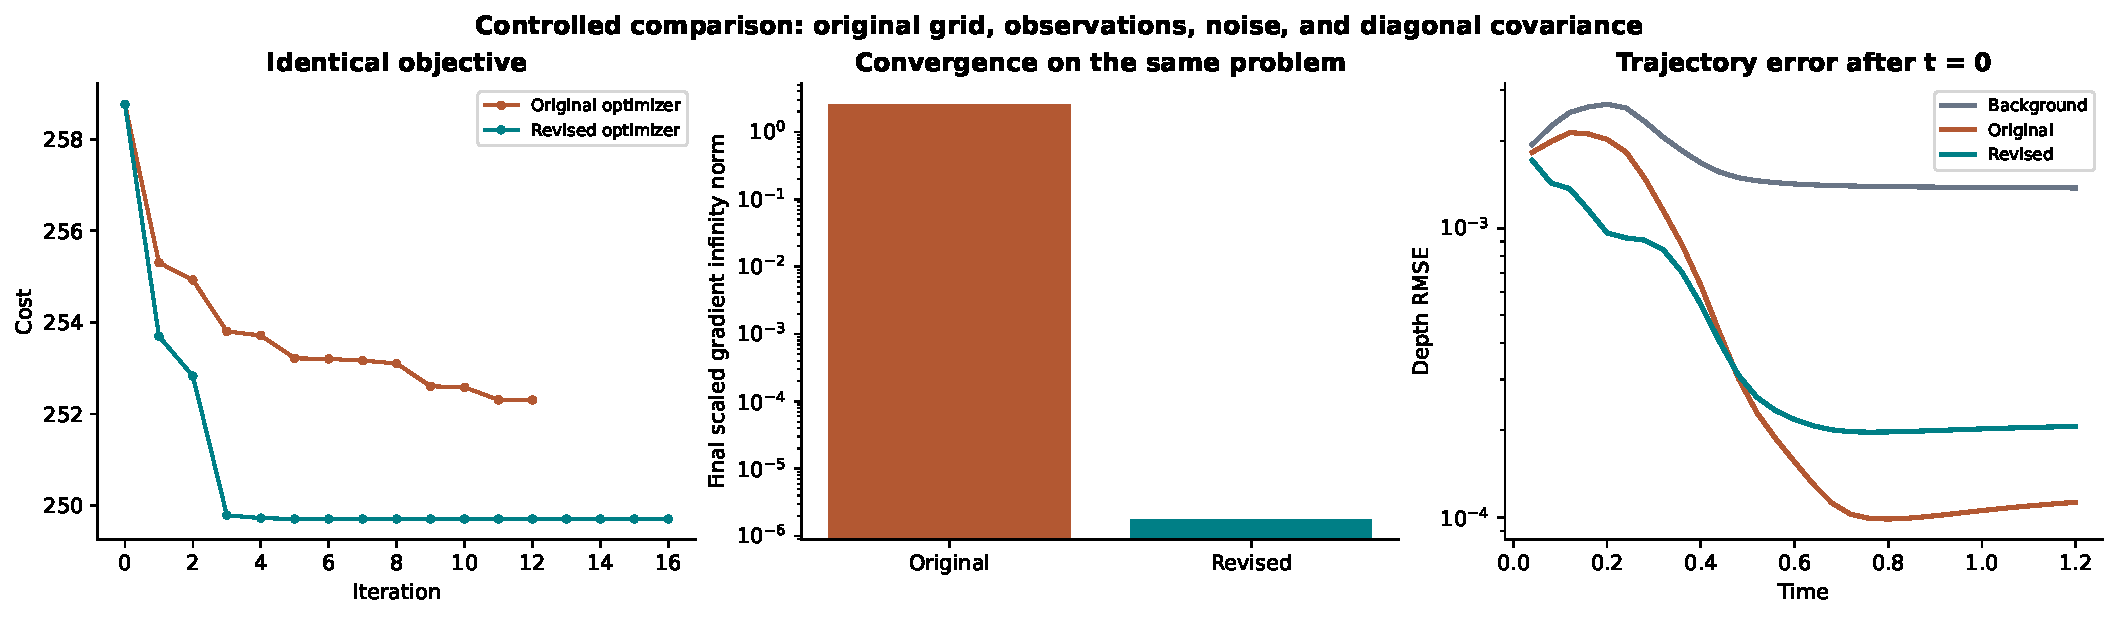
\includegraphics[width=\textwidth]{var_output/baseline_comparison.pdf}
\caption{原始问题不变的对照。左：同一目标函数；中：最终白化梯度无穷范数；
右：$t>0$ 的水深误差。该对照不包含新的相关协方差或更密测点。}
\label{fig:dta-baseline}
\end{figure}

\subsection{相关背景误差孪生实验}

真值初值为
\begin{equation}
 h^\dagger(x,y,0)=1+0.2\exp\left[-\frac{(x-0.5)^2+(y-0.5)^2}{0.02}\right],
 \qquad m_x^\dagger=m_y^\dagger=0.
 \label{eq:dta-truth}
\end{equation}
背景由 $\Q_b=\Q^\dagger(0)+L\boldsymbol\xi_b$ 生成，
$\boldsymbol\xi_b\sim\mathcal N(0,I)$；观测为
$\mathbf y_c=H\Q^{\dagger,n_c}+\sigma_o\boldsymbol\epsilon_c$。
真值和待估轨道使用相同前向模式。

主实验配置见表 \ref{tab:dta-config}。同化测点是规则的 $6\times6$ 格点网络，
每个方向的零基单元索引为 $7,16,25,34,43,52$。
另外在未被同化的单元中随机选择 36 个固定验证测点，使用独立噪声生成验证观测，
这些数据不进入目标函数。背景、训练观测、验证数据的随机种子分别为
20261016、20261017、20261018。

\begin{table}[htbp]
\centering\small
\caption{现行默认实验的运行时参数，来自 \texttt{var\_output/summary.json}。}
\label{tab:dta-config}
\begin{tabular}{ll}
\toprule
参数 & 数值或说明\\
\midrule
区域及网格 & $[0,1]^2$，$60\times60$，$\Delta x=\Delta y=1/60$\\
时间步与观测步距 & $\Delta t=0.001$，$s=20$\\
同化观测时刻 & $C=15$，$t=0.02,0.04,\ldots,0.30$\\
自由预报输出 & 10 个时刻，$t=0.32,0.34,\ldots,0.50$\\
同化／独立验证测点 & 各 36 个，只观测水深\\
观测噪声 & $\sigma_o=0.003$\\
背景标准差 & $\sigma_h=0.03$，$\sigma_{hu}=\sigma_{hv}=0.015$\\
平方根滤波长度 & $\ell=0.06$\\
初值控制维数 & $3N=10800$\\
优化历史长度／上限 & 12／400\\
停止容差 & $\mathrm{gtol}=10^{-5}$，$\mathrm{ftol}=10^{-12}$\\
\bottomrule
\end{tabular}
\end{table}

\subsection{梯度正确性及可接受性结果}

三个完整目标的方向检验见表 \ref{tab:dta-gradient} 和图 \ref{fig:dta-gradient}。
Taylor 斜率由全部九个步长的 $(\log\varepsilon,\log T_\varepsilon)$ 线性拟合得到。
图中保留每个步长的结果，而表中的最小相对误差只概括最佳一致区间。

\begin{table}[htbp]
\centering\small
\caption{完整控制空间目标的三方向检验；全部通过 $2\times10^{-5}$ 阈值。}
\label{tab:dta-gradient}
\begin{tabular}{ccccc}
\toprule
方向 & 伴随方向导数 & 最佳 $\varepsilon$ & 最小相对误差 & Taylor 斜率\\
\midrule
1 & 114.4971754 & $10^{-4}$ & $3.313\times10^{-10}$ & 1.9997\\
2 & 133.4853629 & $10^{-3}$ & $1.292\times10^{-10}$ & 1.9996\\
3 & 48.6344328 & $10^{-2}$ & $1.486\times10^{-9}$ & 1.9993\\
\bottomrule
\end{tabular}
\end{table}

直接 C 测试的 Euler 全状态转置相对误差为 $7.512\times10^{-10}$，
检查点观测梯度的方向误差为 $3.049\times10^{-10}$；开放边界的三个守恒平衡均通过。
六项 Python 回归测试全部通过。对直接 C 内核与检查点反向测试使用
AddressSanitizer 和 UndefinedBehaviorSanitizer，未报告内存或未定义行为错误。
上述为归档版本的测试记录；Tapenade 版本的新增测试另列于前节，二者均不代替网格收敛研究。

\begin{figure}[htbp]
\centering
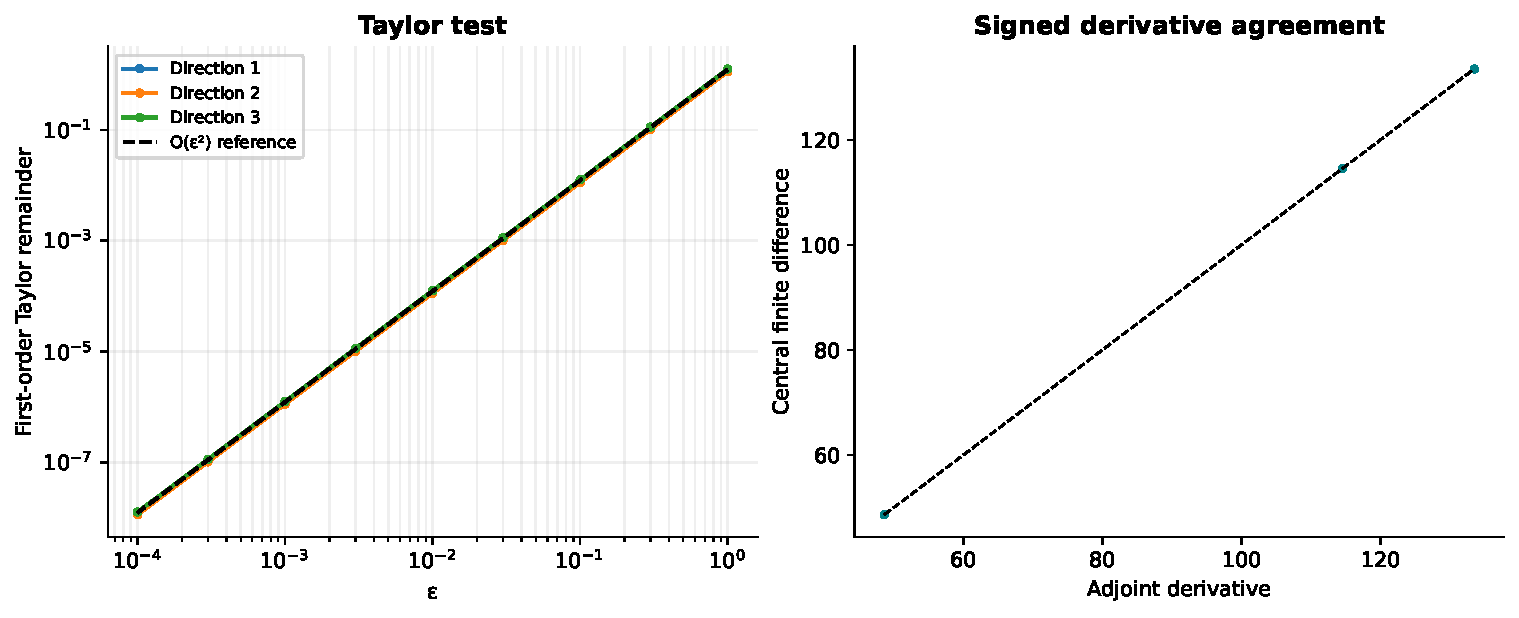
\includegraphics[width=.96\textwidth]{var_output/fd_adjoint_check.pdf}
\caption{完整目标的 Taylor 余项及有符号方向导数比较。左图包含二阶参考线；
右图与对角线重合表示符号和幅度一致。各步长相对误差曲线同时见图 \ref{fig:dta-metrics}。}
\label{fig:dta-gradient}
\end{figure}

所有实验轨道及被检查阶段均保持正水深。真值、背景和分析轨道的最小水深分别为
$0.960831,0.915460,0.959121$，最大二维 CFL 分别为
$0.412677,0.412060,0.413785$，均满足式 \eqref{eq:dta-cfl}。
优化阶段无无效试探，亦无任何状态裁剪。

\subsection{优化收敛结果}

优化接受 305 次更新，记录初始点及终点在内共 306 行历史；优化阶段实际执行
341 次非缓存的目标/梯度求值，\emph{不包含}启动时的有限差分检验。
表 \ref{tab:dta-optimization} 给出初末值。

\begin{table}[htbp]
\centering\small
\caption{相关背景实验的优化收敛，来自 \texttt{cost\_history.csv}。}
\label{tab:dta-optimization}
\begin{tabular}{lrr}
\toprule
指标 & 初始 & 最终\\
\midrule
$J$ & 11809.436264 & 276.464216\\
$J_b=\tfrac12\|\mathbf z\|^2$ & 0 & 43.923318\\
$J_o$ & 11809.436264 & 232.540898\\
$\|\nabla_{\mathbf z}J\|_2$ & $9.80778\times10^3$ & $3.43375\times10^{-4}$\\
$\|\nabla_{\mathbf z}J\|_\infty$ & $1.25025\times10^3$ & $1.48783\times10^{-5}$\\
\bottomrule
\end{tabular}
\end{table}

SciPy 的成功退出原因为相对目标下降满足式 \eqref{eq:dta-stopping}，
并非无穷范数已经低于 $10^{-5}$；最终梯度仍接近该阈值。
总代价降低 $97.66\%$。梯度范数不必单调，背景惩罚也可随拟合改善而上升。
完整实验计算阶段耗时约 168.2 秒，包含梯度检查和保存结果，不含随后绘图；
环境为 Python 3.12.3、NumPy 1.26.4、SciPy 1.13.1，时间只代表当前机器上的这次运行。

\begin{figure}[htbp]
\centering
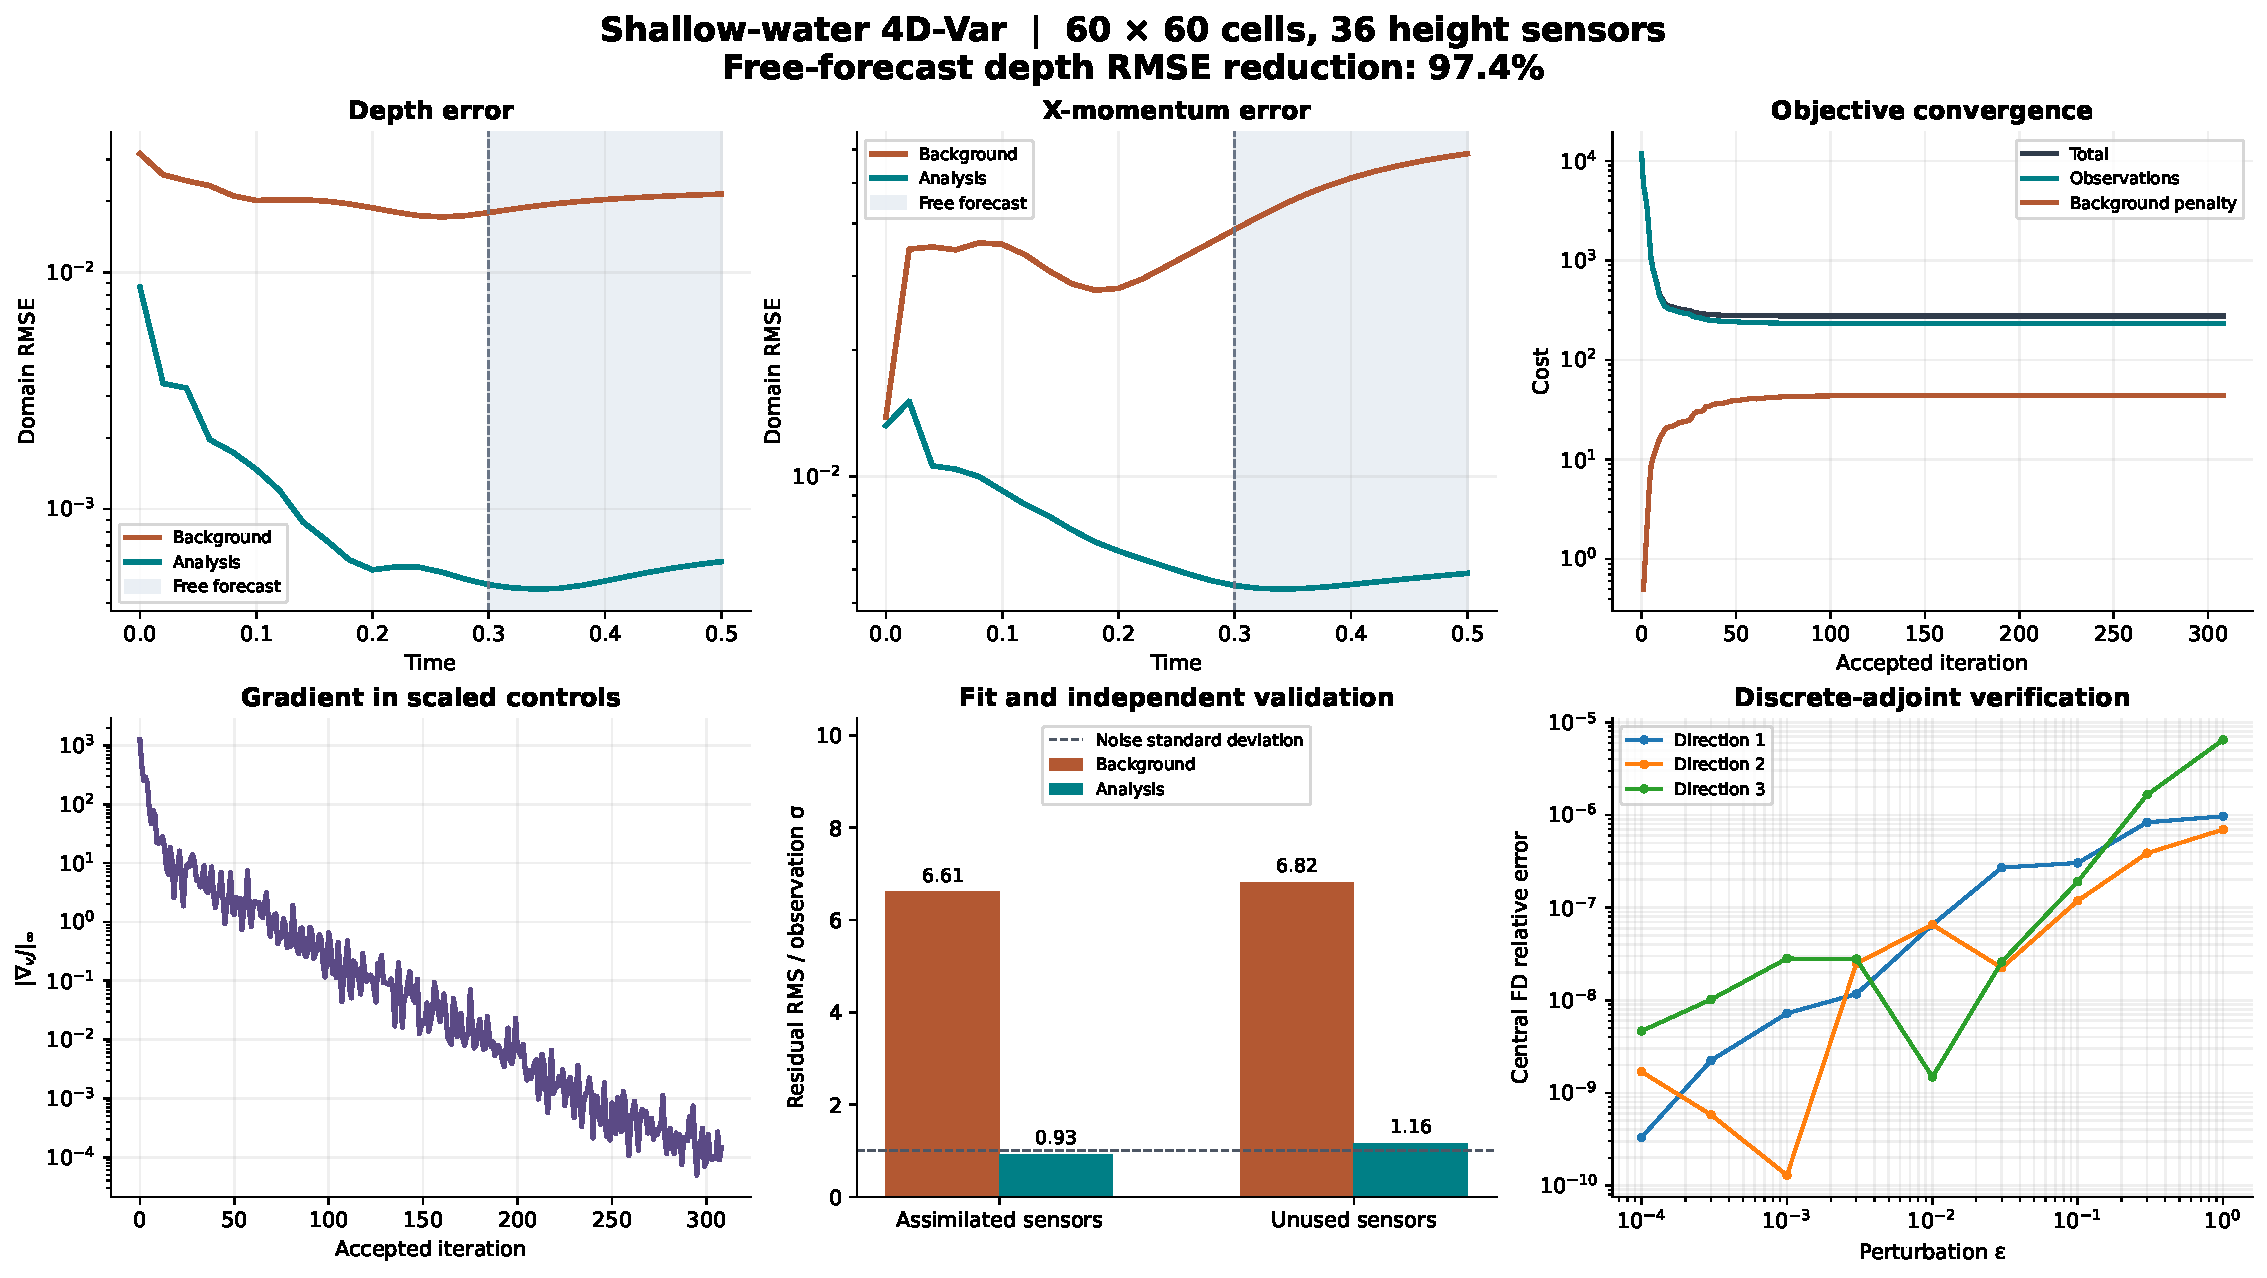
\includegraphics[width=\textwidth]{var_output/var_4d_metrics.pdf}
\caption{相关背景实验的总体诊断：水深和 $x$ 动量轨道误差、代价、白化梯度、
训练和独立验证测点残差，以及三方向梯度检验。轨道图的阴影区位于同化窗外，未使用观测。}
\label{fig:dta-metrics}
\end{figure}

\subsection{误差指标、窗内恢复与独立自由预报}

对单个物理分量 $r$，时刻误差定义为
\begin{equation}
 \mathrm{RMSE}_r(t_c)=
 \left[\frac1N\sum_{i,j}(q_{r,i,j}(t_c)-q^\dagger_{r,i,j}(t_c))^2\right]^{1/2}.
 \label{eq:dta-time-rmse}
\end{equation}
对输出时刻集合 $\mathcal T$ 的整体误差为
\begin{equation}
 \mathrm{RMSE}_{r,\mathcal T}=
 \left[\frac{1}{|\mathcal T|N}\sum_{t_c\in\mathcal T}\sum_{i,j}
 (q_{r,i,j}(t_c)-q^\dagger_{r,i,j}(t_c))^2\right]^{1/2},\qquad
 \rho_{r,\mathcal T}=1-\frac{\mathrm{RMSE}_{r,\mathcal T}^{a}}
                              {\mathrm{RMSE}_{r,\mathcal T}^{b}}.
 \label{eq:dta-window-rmse}
\end{equation}
这是先汇总平方误差再开方，不是各时刻 RMSE 比值的平均。
同化统计使用 $\mathcal T_a=\{0,0.02,\ldots,0.30\}$，包括初值；
预报统计只使用 $\mathcal T_f=\{0.32,0.34,\ldots,0.50\}$。

\begin{table}[htbp]
\centering\small
\caption{相关背景实验的全场 RMSE。预报统计严格位于最后观测时刻之后。}
\label{tab:dta-rmse}
\begin{tabular}{llrrr}
\toprule
区间 & 分量 & 背景 & 分析 & 降低率\\
\midrule
初始时刻 & $h$ & 0.0317399 & 0.00866902 & $72.69\%$\\
\midrule
同化窗（含初值） & $h$ & 0.0211449 & 0.00263436 & $87.54\%$\\
 & $hu$ & 0.0322686 & 0.00890184 & $72.41\%$\\
 & $hv$ & 0.0423474 & 0.00827857 & $80.45\%$\\
\midrule
窗外自由预报 & $h$ & 0.0202920 & 0.000518382 & $97.45\%$\\
 & $hu$ & 0.0516189 & 0.00559197 & $89.17\%$\\
 & $hv$ & 0.0550445 & 0.00541035 & $90.17\%$\\
\bottomrule
\end{tabular}
\end{table}

图 \ref{fig:dta-components} 展示三个分量的时间演化。虽然只同化水深，动量通过模型的
通量耦合获得约束，但这不意味着全部动量模态都能从稀疏水深观测唯一确定。
图 \ref{fig:dta-fields} 用一致的水深色标及共享的对称误差色标比较初值、窗口末端和
预报末端，不把背景减分析的修正量误称为相对真值的误差降低。

\begin{figure}[htbp]
\centering
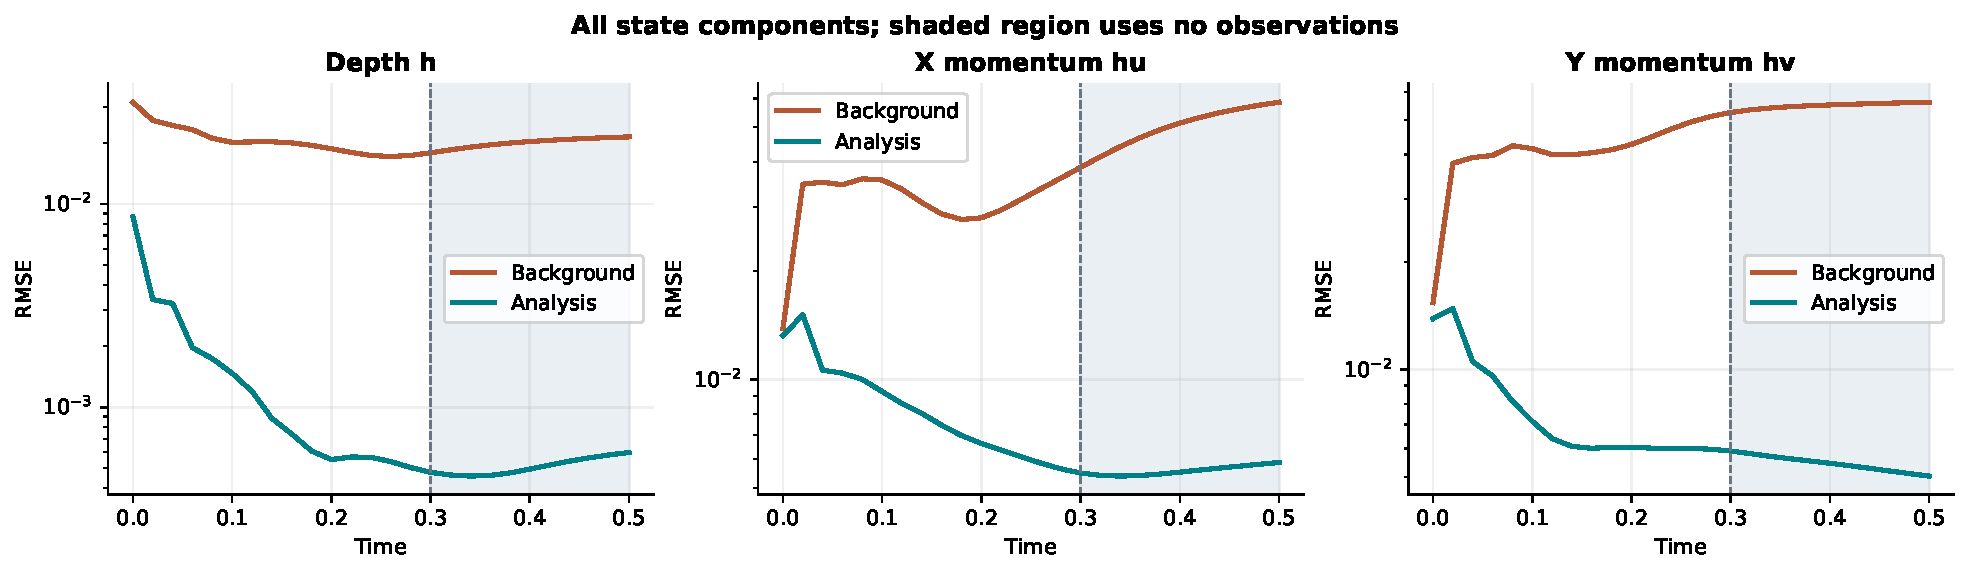
\includegraphics[width=\textwidth]{var_output/all_components_rmse.pdf}
\caption{三个守恒分量的背景与分析轨道误差。$t=0.30$ 后为不使用观测的自由预报。
曲线在同化窗内对应平滑重建，在窗外才构成独立时间外推验证。}
\label{fig:dta-components}
\end{figure}

\begin{figure}[p]
\centering
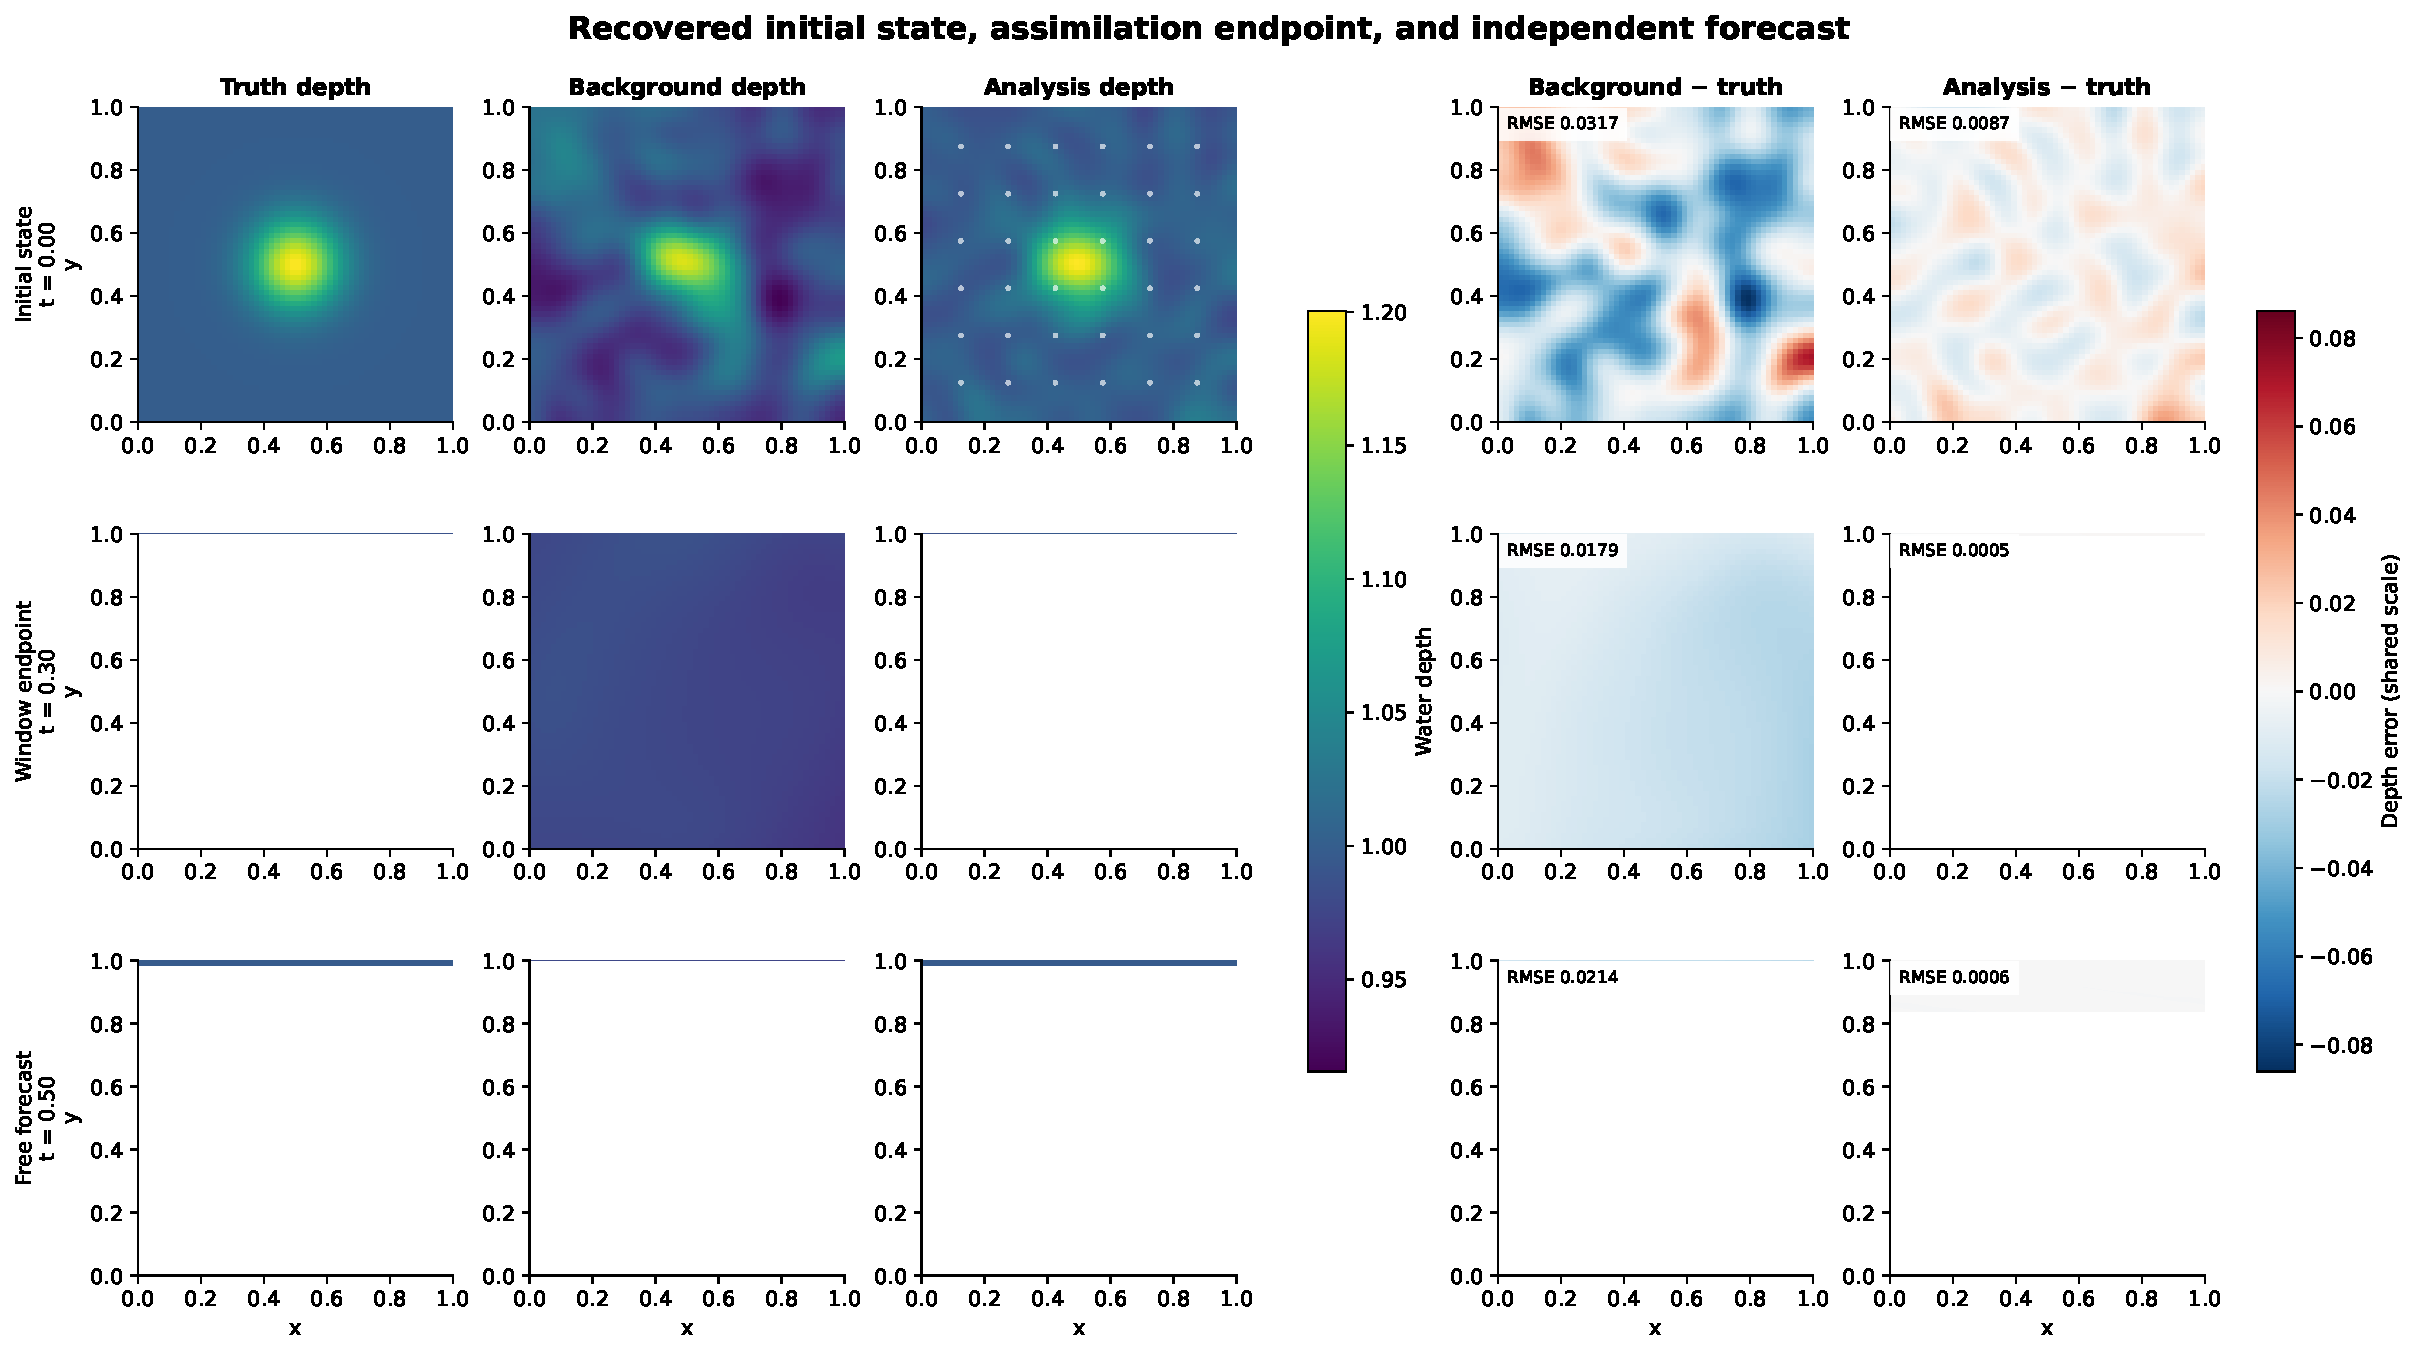
\includegraphics[width=\textwidth]{var_output/var_4d_snapshots.pdf}
\caption{从上到下为 $t=0,0.30,0.50$；从左到右为真值、背景、分析、水深背景误差和分析误差。
白点标记同化测点，两个误差列使用相同色标。初始水深结构得到恢复；后期波动已部分离开
开放区域，分析同时纠正了背景中的持续偏移。}
\label{fig:dta-fields}
\end{figure}

\subsection{独立测点检验与解释边界}

训练和验证残差均按相同的 15 个时刻及各自的 36 个测点计算
\begin{equation}
 \mathrm{RMS}_{\mathrm{obs}}=
 \left[\frac1{CM}\sum_{c,p}(h_{o_p}(t_c)-y_{c,p})^2\right]^{1/2}.
 \label{eq:dta-observation-rms}
\end{equation}
这里包含观测噪声，与全场相对无噪真值的 RMSE 不是同一个指标。
\begin{table}[htbp]
\centering\small
\caption{观测空间检验。独立测点及其噪声均不参与优化。}
\label{tab:dta-heldout}
\begin{tabular}{lrrrr}
\toprule
测点集合 & 背景 RMS & 分析 RMS & 分析 RMS/$\sigma_o$ & 降低率\\
\midrule
同化测点 & 0.0198406 & 0.00278413 & 0.9280 & $85.97\%$\\
独立测点 & 0.0204450 & 0.00349414 & 1.1647 & $82.91\%$\\
\bottomrule
\end{tabular}
\end{table}

这些结果表明改进不只发生在被直接拟合的空间位置，且在窗外仍有明显收益。
但本实验的真值与反演模式相同，背景误差按所用 $B$ 生成，也没有模型误差或观测偏差。
开放边界允许初始重力波离开区域，较大的后期改善率部分来自对背景持续偏移的纠正。
不能据此推断真实数据、复杂地形、湿干问题或不同误差统计下也有相同收益。
此外尚未开展网格／时间步收敛、多随机种子统计或失配协方差的系统研究。

\clearpage
\section{Tapenade 二项式伴随的独立验证与重跑结果}
\label{sec:dta-tapenade-results}

现行自动生成版本保持上述 $60\times60$ 孪生实验的配置、随机种子、观测和先验不变，
以 8 个二项式快照槽重新执行完整优化与窗外预报。
本节归档结果来自含调度计数器的早期 Tapenade 版本，保存于 \path{var_output_tapenade/}；此前 \path{var_output/} 的文件未被覆盖。
对生成器的机械修复、运行时对齐修复和源代码校验均已纳入可复现流程。

\subsection{相同初值处的导数与检查点预算比较}

先在归档实验的背景初值及归档分析初值处，直接比较自动生成和手工伴随对同一 $J_o$
给出的完整 $10800$ 维梯度。预算 $1,2,4,8,16$ 下，两种代价逐位相同；
梯度相对二范数误差分别为背景处 $3.105\times10^{-16}$、分析处 $1.687\times10^{-15}$，
所有预算均得到相同梯度。每次逆转恰好 300 步，反向结束时字节磁带计数均为零。
因此存储预算只改变重算安排，不改变观测目标或其离散导数。

\begin{table}[htbp]
\centering\small
\caption{300 步、$60\times60$ 模型的实测二项式调度。
有效载荷不含局部磁带、工作数组或内存分配块开销。}
\label{tab:dta-binomial}
\begin{tabular}{rrrr}
\toprule
快照预算 & 实测峰值快照数 & 调度前向 RK2 步数 & 快照有效载荷（MB）\\
\midrule
1 & 1 & 45150 & 0.259212\\
2 & 2 & 4900 & 0.518424\\
4 & 4 & 1938 & 1.036848\\
8 & 8 & 1280 & 2.073696\\
16 & 16 & 1029 & 4.147392\\
\bottomrule
\end{tabular}
\end{table}

上述调度计数不包括验证积分的 300 步及每个局部反向 RK2 内部的一次 Euler 重算。
预算 8 时，背景处的单次生成梯度求值约为 $1.13$ s，手工参考约为 $0.49$ s；
这是有并发实验负载时的单次测量，不是严格的性能基准。
采用自动微分的目的在于从前向代码生成一致的伴随，并提供可调存储预算，
不能将其解释为运行速度必然优于专门优化的手工实现。

\begin{figure}[htbp]
\centering
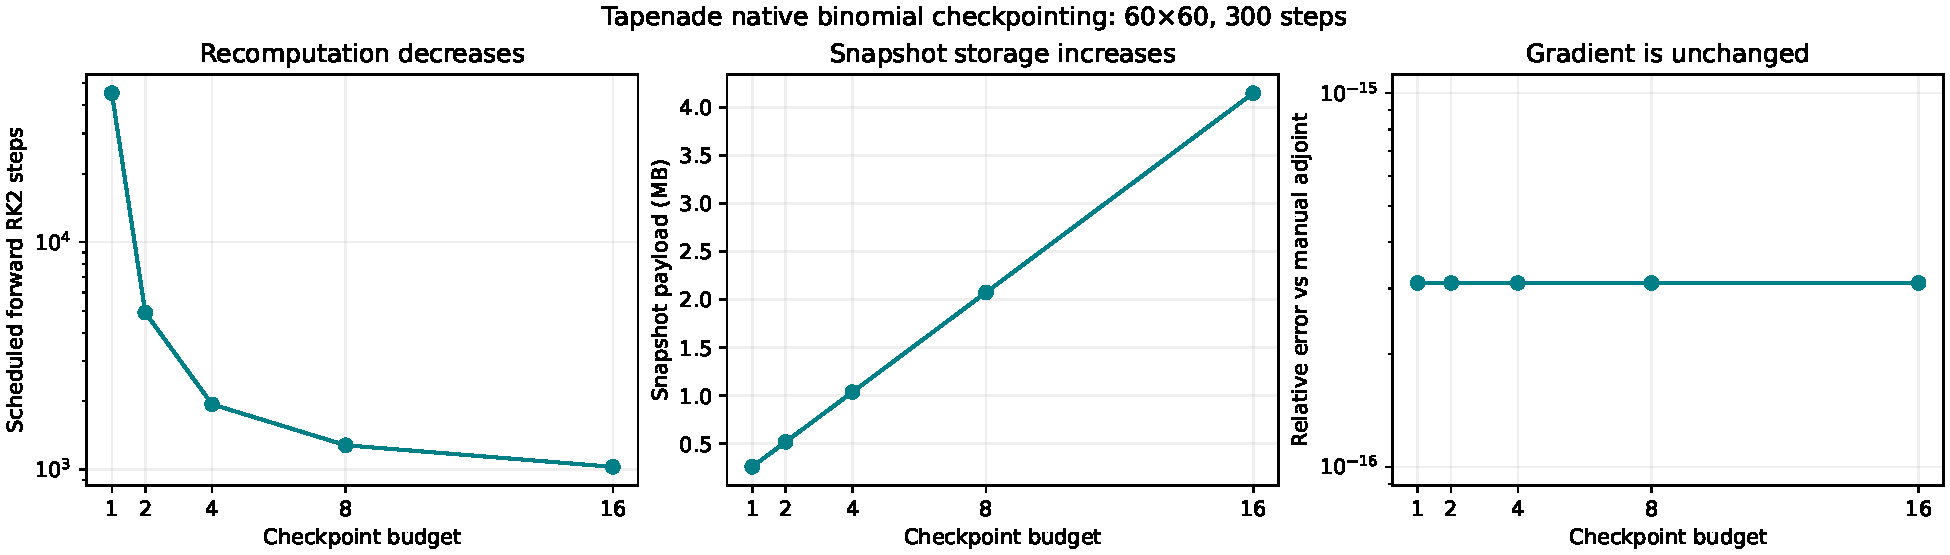
\includegraphics[width=\textwidth]{var_output_tapenade/checkpoint_tradeoff.pdf}
\caption{Tapenade 原生二项式调度的实测存储／重算权衡。
各预算得到相同梯度；右图比较背景处的完整梯度与手工参照。}
\label{fig:dta-binomial}
\end{figure}

\subsection{完整 4D-Var 重新运行}

自动生成版本接受 309 次迭代，执行 345 次非缓存优化求值，无无效试探。
运行约 $356.2$ s，包含启动时的梯度验证，但不含随后绘图。
退出原因为相对代价下降满足容差，最终梯度无穷范数仍高于 $10^{-5}$ 的梯度阈值，
因此不能称为通过该梯度停止准则。三方向完整目标检验的最佳相对误差为
$3.313\times10^{-10}$、$1.292\times10^{-10}$、$1.486\times10^{-9}$。

\begin{table}[htbp]
\centering\small
\caption{Tapenade C 伴随与 8 个二项式快照槽的重新运行结果。}
\label{tab:dta-tapenade-run}
\begin{tabular}{lrr}
\toprule
指标 & 初始／背景 & 最终／分析\\
\midrule
完整目标 $J$ & 11809.436263851 & 276.464216016\\
最终 $\|\nabla_{\mathbf z}J\|_\infty$ & --- & $2.42925\times10^{-5}$\\
窗内时空水深 RMSE（含初值） & 0.02114487 & 0.002634356\\
窗外自由预报水深 RMSE & 0.02029201 & 0.0005183793\\
训练测点残差 RMS & 0.01984056 & 0.002784127\\
独立测点残差 RMS & 0.02044503 & 0.003494142\\
\bottomrule
\end{tabular}
\end{table}

窗内和窗外水深 RMSE 分别降低约 $87.5\%$ 和 $97.4\%$，独立测点残差降低约 $82.9\%$。
新旧完整优化的最终代价差约为 $2.62\times10^{-10}$。
逆序求和的浮点舍入差异可以改变 L-BFGS 的细节及停止迭代数，
故不要求整个优化历史逐位一致；相同状态处的目标与梯度比较提供更直接的实现一致性证据。
分析轨道最小水深为 $0.959121$，最大二维 CFL 为 $0.413785$，均满足可接受性条件。

\begin{figure}[htbp]
\centering
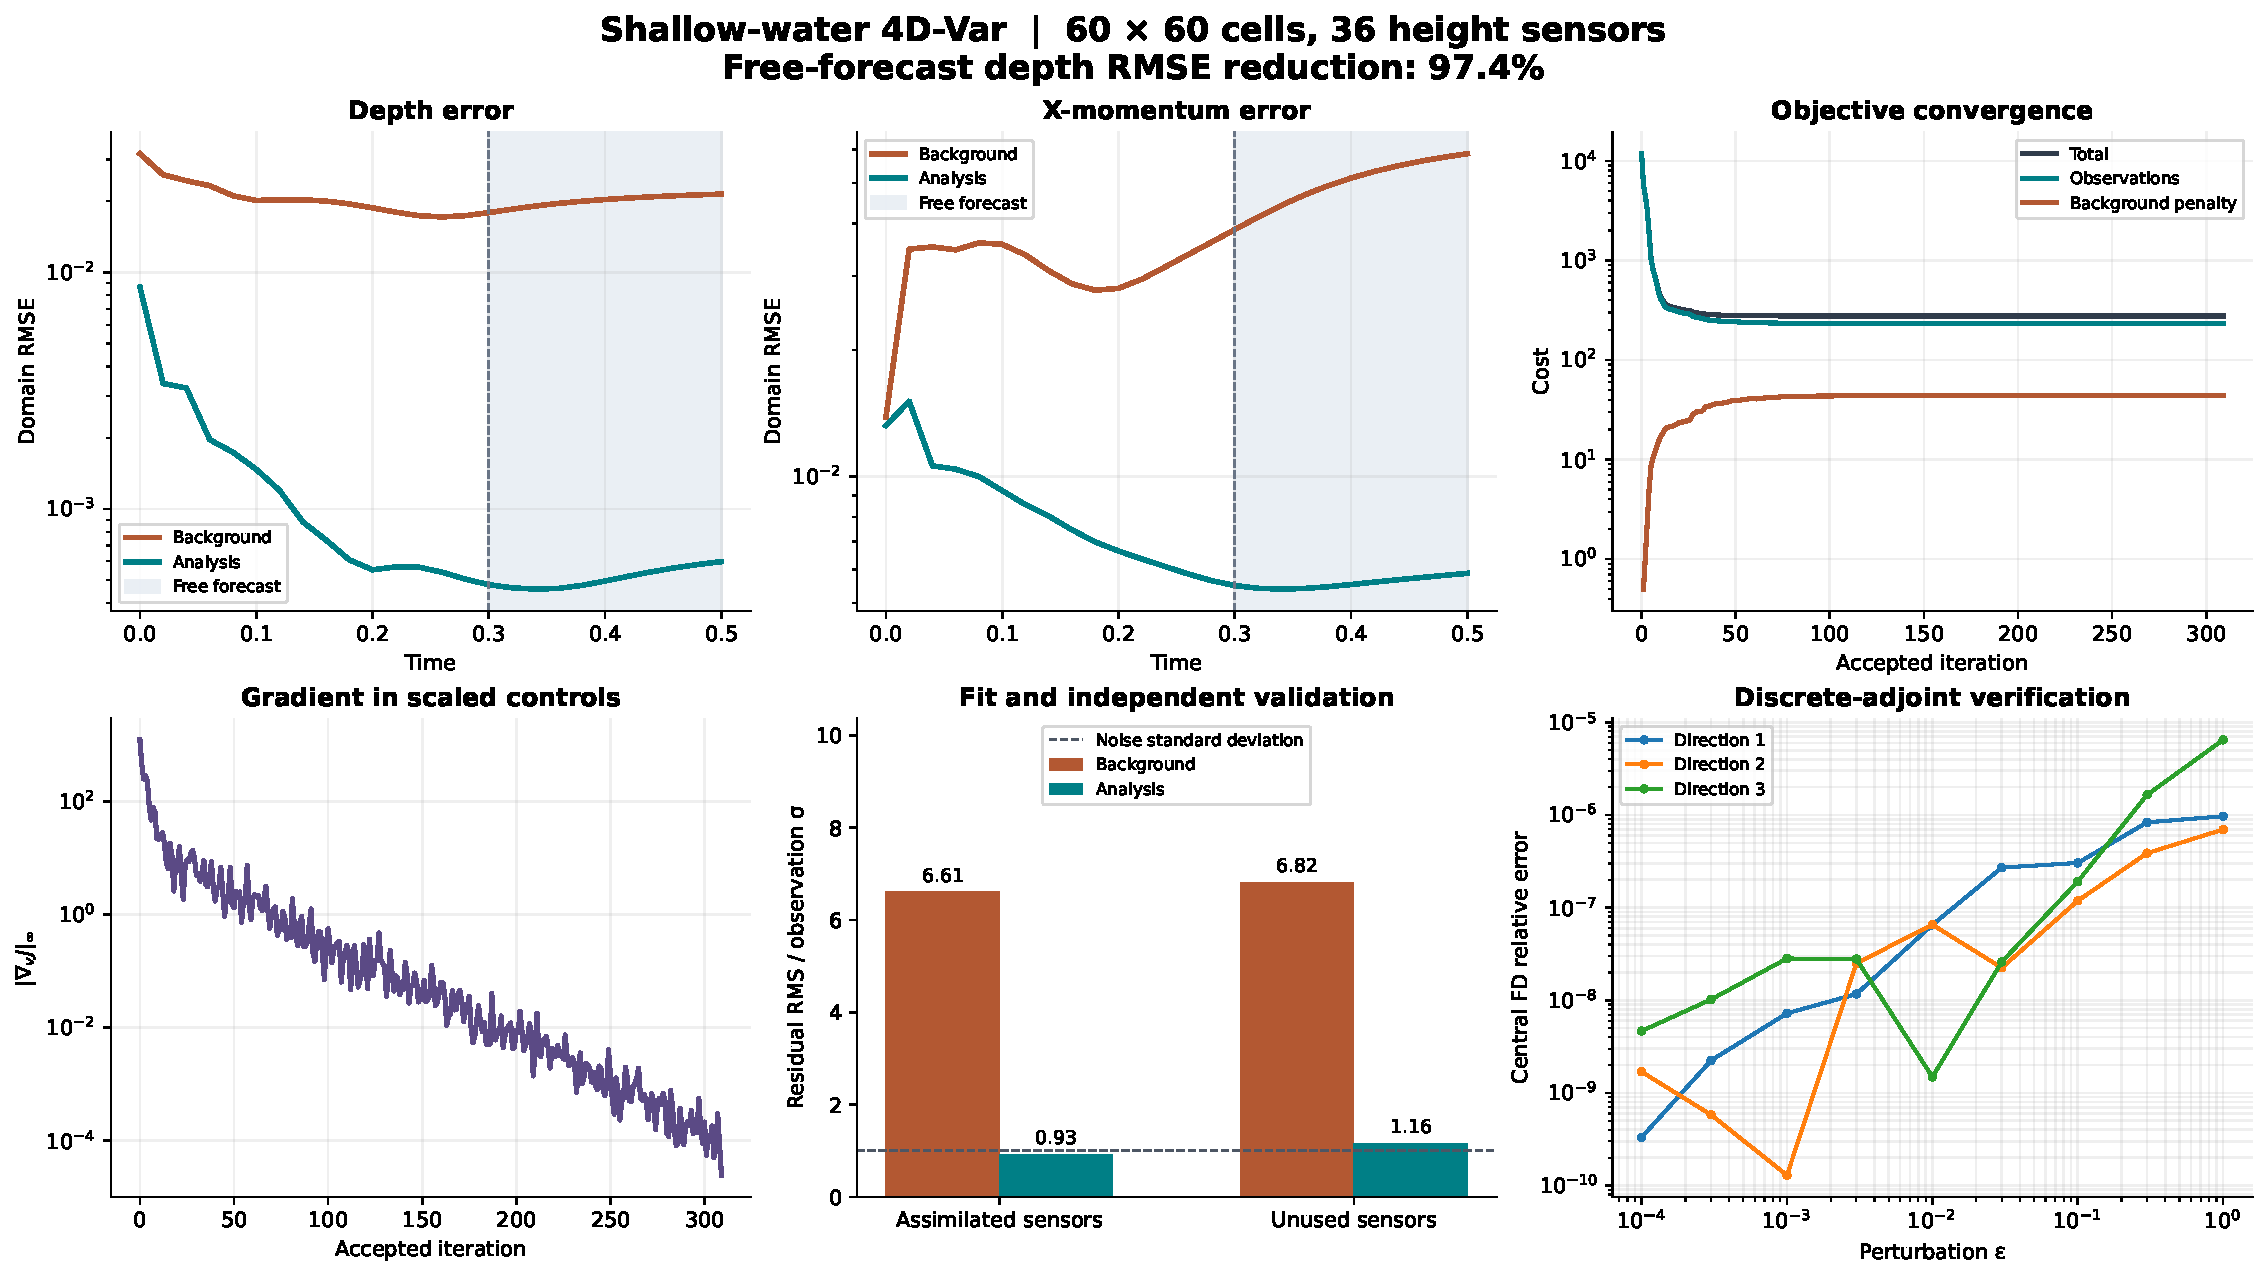
\includegraphics[width=\textwidth]{var_output_tapenade/var_4d_metrics.pdf}
\caption{使用 Tapenade 生成的 C 伴随重新运行的完整实验。
包含目标收敛、梯度、未参与同化的测点以及窗外自由预报。}
\label{fig:dta-tapenade-metrics}
\end{figure}

\section{可复现运行与结果追踪}
\label{sec:dta-reproducibility}

现行 Tapenade 版本的生成、验证和运行命令为
\begin{verbatim}
make generate-adjoint TAPENADE=/path/to/tapenade
make test
make sanitize
python3 assimilate.py --checkpoint-budget 8 --output var_output_tapenade
python3 plot_4dvar_result.py --output var_output_tapenade --movie
python3 benchmark_checkpointing.py \
  --reference var_output \
  --output var_output_tapenade
\end{verbatim}
生成源代码保存在 \path{tapenade_out/}，普通构建不运行 Tapenade。
运行时从已安装工具包的 \path{ADFirstAidKit/} 读取，构建脚本仅在
\path{build/tapenade_runtime/} 中复制、应用对齐补丁并编译，不修改工具包安装。
工具包位置可通过 \texttt{TAPENADE\_HOME} 设置；临时生成输入与原始输出位于
\path{build/tapenade-generation/}，可由 \texttt{make clean} 清理。
修改前向算术后必须重新生成；普通构建检查源代码哈希以防使用过期伴随。
\path{var_output_tapenade/summary.json} 记录新实验的配置、实际后端、检查点预算、
优化退出原因及数值源文件哈希；同目录的 \path{checkpoint_benchmark.csv}
保存各预算在背景和归档分析处的导数比较与计数。

默认主实验执行
\begin{verbatim}
bash run.sh
\end{verbatim}
该脚本编译 C 共享库，运行 Python 与 C 数值测试，执行主实验并保存静态图和动画。
可分别运行
\begin{verbatim}
python3 assimilate.py --help
python3 assimilate.py --output var_output
python3 plot_4dvar_result.py --output var_output --movie
make test
\end{verbatim}
本次主实验输出如下：
\begin{itemize}
 \item \path{var_output/summary.json}：配置、成功标志、退出原因、误差统计、阶段诊断、
       运行环境和数值源代码 SHA-256。
 \item \path{var_output/experiment.npz}：真值、背景、分析轨道，坐标、时刻、训练／验证
       观测及最终控制。状态数组顺序为 $(\text{time},3,N_y,N_x)$，分量顺序为 $(h,hu,hv)$。
 \item \path{cost_history.csv}、\path{trajectory_metrics.csv}、\path{gradient_check.csv}：
       逐接受迭代、逐输出时刻及逐扰动步长的诊断；三个文件均位于 \path{var_output/}。
 \item 本文引用四幅主实验静态图及一幅原问题对照图，文件为
       \path{baseline_comparison.pdf}、\path{fd_adjoint_check.pdf}、\path{var_4d_metrics.pdf}、
       \path{all_components_rmse.pdf}、\path{var_4d_snapshots.pdf}；均在 \path{var_output/}，
       并各有 PNG 版本。\path{var_4d_result.gif} 按物理时间播放，不把优化迭代混作时间步。
\end{itemize}

\section{小结}

现行 DTA 方法对实际执行的有限体积、开放边界和 RK2 组合逐项求导，
由 Tapenade 自动生成 C 伴随，以原生二项式检查点重算提供精确的局部线性化状态，并以
$\nabla_{\mathbf z}J=\mathbf z+L\trans\LL^0$ 连接观测伴随与白化背景先验。
局部转置、守恒、全目标方向导数和 Taylor 检验共同支持梯度的一致性；
相同问题的对照支持优化器修正的有效性；独立测点和窗外自由预报则检验了新孪生实验的
重建收益。优化正确性、观测可辨识性和模型对现实的适用性是不同层次的问题，
应分别由对应证据判断。

\bibliographystyle{plain}
\bibliography{ref}
\end{document}
